\begin{frame}{How DiscoNet Works}
  \SlideBody{\begin{VisualCanvas}
    \node[visual title] at (0,5.7) {DiscoNet: Distilled Collaboration Network};
    % Centers of the original figure's input boxes, scaled with its height.
    \node[visual label,anchor=north] at ({0.10+144.30*4.05/680.40},5.07) {Student};
    \node[visual label,anchor=north] at ({0.10+633.18*4.05/680.40},5.07) {Teacher};
    \node[anchor=north west,inner sep=0] at (0.10,4.62)
      {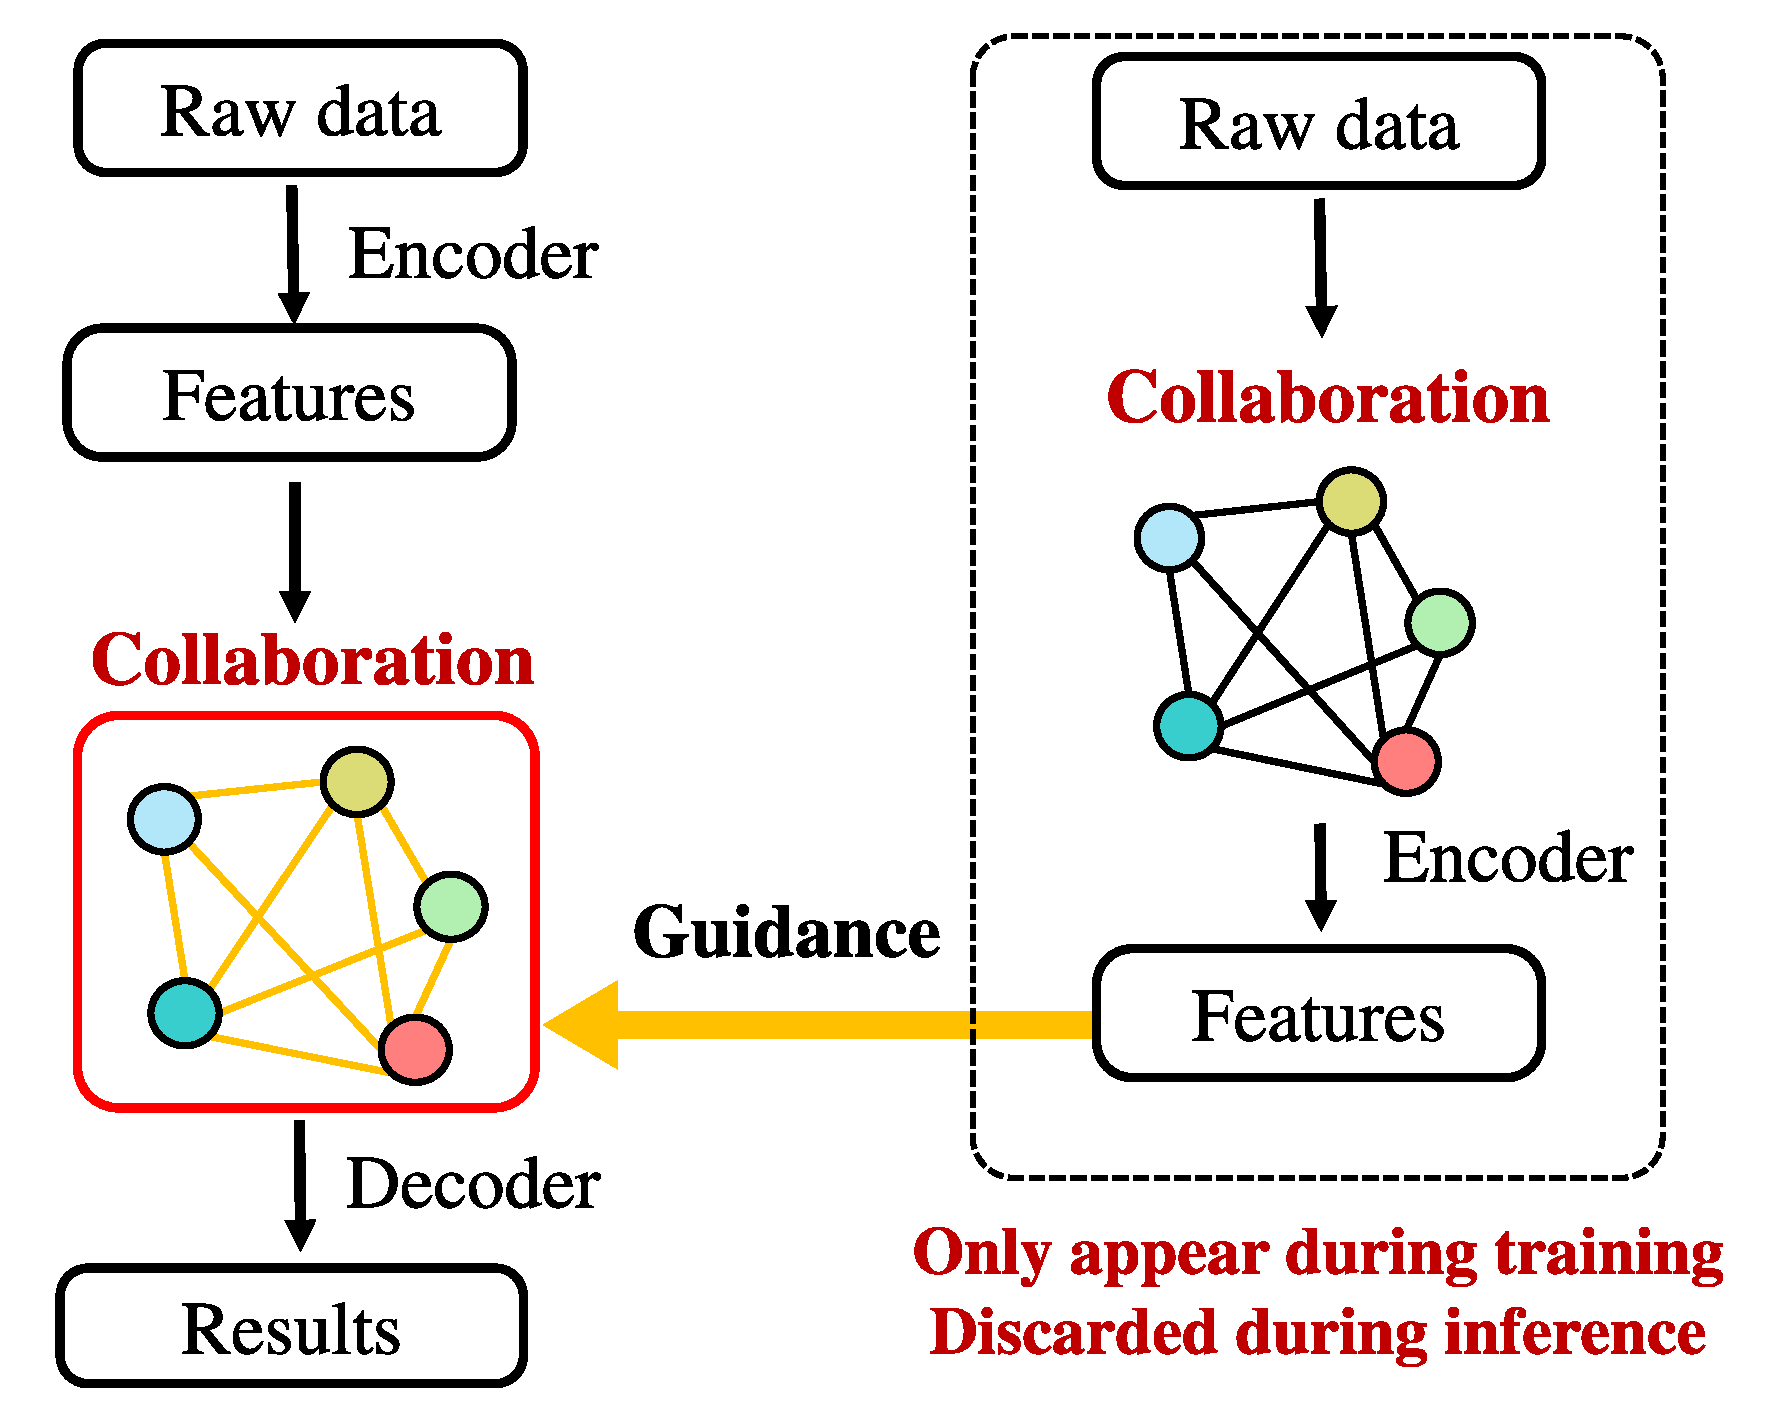
\includegraphics[height=4.05cm]{assets/papers/disconet/fig1_ours.pdf}};
    \node[visual label] at (6.0,5.05) {Feature Exchange and Spatial Attention};
    \node[anchor=north west,inner sep=0] at (6.0,4.52)
      {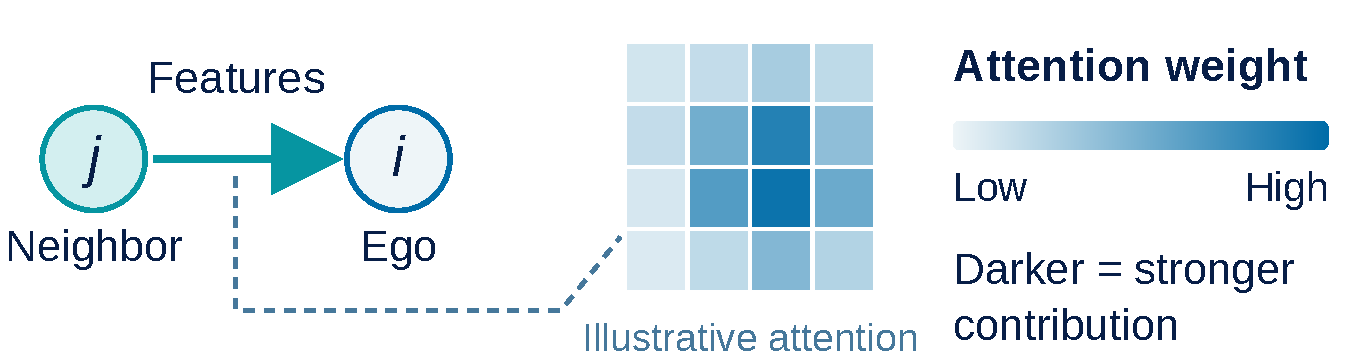
\includegraphics[width=8.65cm]{assets/diagrams/edge-weights.pdf}};
    \node[visual text,text width=8.65cm] at (6.0,2.00)
      {Share learned BEV features.\par Compute attention matrices at the receiver.};
    \node[visual label] at (6.0,0.99) {Knowledge Distillation (KD)};
    \node[visual text,text width=8.65cm] at (6.0,0.55)
      {The teacher guides student features\par during training.};
  \end{VisualCanvas}}
  \SlideSource{Source: \href{https://arxiv.org/html/2111.00643v2\#S1.F1}{Li et al., Fig. 1(c)}.}
\end{frame}
